\section{Computational Cryptography}


To introduce computational cryptography we first have to define a computational model.
We assume the adversary is efficient, \ie it is a \ac{PPT} adversary.

We want that the probability of success of the adversary is tiny, \ie negligible for some $\lambda \in \NaturalsZ$.
A function $\epsilon : \NaturalsZ \to \Reals$ is negligible if $\forall c > 0 . \exists n_0$ such that $\forall n > n_0 . \epsilon(n) < n^{-c}$.

We rely on computational assumptions, \ie in tasks believed to be hard for any efficient adversary.
In this setting we make conditional statements, \ie if a certain assumption holds then a certain crypto-scheme is secure.

\subsection{\aclp{OWF}}

A simple computational assumption is the existence of \acp{OWF}, \ie functions for which is hard to compute the inverse.

\begin{definition}[\acl{OWF}]
	A function $f : \{0,1\}^{\star} \to \{0,1\}^{\star}$ is a \ac{OWF} if $f(x)$ can be computed in polynomial time for all $x$ and for all $\ac{PPT}$ adversaries $\Adv$ it holds that
	\begin{equation*}
		\Pr{f(x') = y : x \rand{\{0,1\}^{\star}}; \; y = f(x); \; x' \from \Adv(1^{\lambda}, y)} \le \epsilon(\lambda). \qedhere
	\end{equation*}
\end{definition}

The $1^{\lambda}$ given to the adversary $\Adv$ is there to highlight the fact that $\Adv$ is polynomial in the length of the input ($\lambda$).

Russel Impagliazzo proved that \acp{OWF} are equivalent to One Way Puzzles, \ie couples $(\mathrm{Pgen}, \mathrm{Pver})$ where $\mathrm{Pgen}(1^{\lambda}) \to (y, x)$ gives us a puzzle ($y$) and a solution to it ($x$), while $\mathrm{Pver}(x,y) \to 0/1$ verifies if $x$ is a solution of $y$.

Another object of interest in this classification are average hard NP-puzzles, for which you can only get an instance, \ie $\mathrm{Pgen}(1^{\lambda}) \to y$.

Impagliazzo says we live in one of five worlds:
\begin{enumerate}
	\item Algorithmica, where P = NP;
	\item Heuristica, where there are no average hard NP-puzzles, \ie problems without solution;
	\item Pessiland, where you have average hard NP-puzzles;
	\item Minicrypt, where you have \ac{OWF}, one-way NP-puzzles, but no \ac{PKC};
	\item Cryptomania, where you have both \ac{OWF} and \ac{PKC}.
\end{enumerate}
We'll stay in Minicrypt for now.

\ac{OWF} are hard to invert on average.
Two examples:
\begin{itemize}
	\item factoring the product of two large prime numbers;
	\item compute the discrete logarithm, \ie take a finite group $(\Group, \cdot)$, and compute $y = g^x$ for some $g \in \Group$.
	The find $x = \log_{g}(y)$.
	This is hard to compute in some groups, \eg $\IntegersPrimeGroup$.
\end{itemize}

\subsection{Computational Indistinguishability}

\begin{definition}[Distribution Ensemble]
	A distribution ensemble $\X = \{ X_n \}_{n \in \NaturalsZ}$ is a sequence of distributions $X_i$ over some space $\{0,1\}^{\lambda}$.
\end{definition}

\begin{definition}[Computational Indistinguishability]
	Two distribution ensembles $\X_{\lambda}$ and $\Y_{\lambda}$ are computationally indistinguishable, written as $\X_{\lambda} \CompInd \Y_{\lambda}$, if for all \ac{PPT} distinguishers $\Distinguisher$ it holds that
	\begin{equation*}
		\abs{\Pr{\Distinguisher(\X_{\lambda}) = 1} - \Pr{\Distinguisher(\Y_{\lambda}) = 1}} \le \epsilon(\lambda).
	\end{equation*}
\end{definition}

\begin{lemma}[Reduction] \label{lem:reduction}
	If $\X \CompInd \Y$, then for all \ac{PPT} functions $f$, $f(\X) \CompInd f(\Y)$.
\end{lemma}

\begin{proof}[Proof of \cref{lem:reduction}]
	Assume, for the sake of contradiction, that $\exists f$ such that $f(\X) \not \CompInd f(\Y)$: then we can distinguish $\X$ and $\Y$.
	Since $f(\X) \not \CompInd f(\Y)$, then $\exists p = \poly(\lambda), \Distinguisher$ such that, for infinitely many $\lambda$s
	\begin{equation*}
		\abs{\Pr{\Distinguisher(f(\X_{\lambda})) = 1} - \Pr{\Distinguisher(f(\Y_{\lambda})) = 1}} \ge \frac{1}{p(\lambda)}.
	\end{equation*}

	$\Distinguisher$ distinguishes $\X_{\lambda}$ and $\Y_{\lambda}$ with non-negligible probability.
	Consider the following $\Distinguisher'$, which is given
	\begin{equation*}
		z =
		\begin{cases}
			x \rand{\X_{\lambda}}; \\
			y \rand{\Y_{\lambda}}. \\
		\end{cases}
	\end{equation*}
	$\Distinguisher'$ runs $\Distinguisher(f(z))$ and outputs whatever it outputs, and has the same probability of distinguishing $\X$ and $\Y$ of $\Distinguisher$, in contradiction with the fact that $\X \CompInd \Y$.
\end{proof}

Now we show that computational indistinguishability is transitive.

\begin{lemma}[Hybrid Argument] \label{lem:hybrid-argument}
	Let $\X = \{X_{\lambda}\}$, $\Y = \{ Y_{\lambda} \}$, $\Z = \{ Z_{\lambda} \}$ be distribution ensembles.
	If $\X_{\lambda} \CompInd \Y_{\lambda}$ and $\Y_{\lambda} \CompInd \Z_{\lambda}$, then $\X_{\lambda} \CompInd \Z_{\lambda}$.
\end{lemma}

\begin{proof}[Proof of \cref{lem:hybrid-argument}]
	This follows from the triangular inequality.
	\begin{align*}
		\abs{\Pr{\Distinguisher(\X_{\lambda}) = 1} - \Pr{\Distinguisher(\Z_{\lambda}) = 1}}
		= &~
		\left| \Pr{\Distinguisher(\X_{\lambda}) = 1} - \Pr{\Distinguisher(\Y_{\lambda}) = 1} \right.
		\\
		&~+
		\left. \Pr{\Distinguisher(\Y_{\lambda}) = 1} - \Pr{\Distinguisher(\Z_{\lambda}) = 1} \right|
		\\
		\le &~
		\abs{\Pr{\Distinguisher(\X_{\lambda}) = 1} - \Pr{\Distinguisher(\Y_{\lambda}) = 1}}
		\\
		&~+
		\abs{\Pr{\Distinguisher(\Y_{\lambda}) = 1} - \Pr{\Distinguisher(\Z_{\lambda}) = 1}}
		\\
		\le &~2 \epsilon(\lambda). \tag{negligible}
	\end{align*}
\end{proof}

We often prove $\X \CompInd \Y$ by defining a sequence $\H_0, \H_1, \dots, \H_t$ of distributions ensembles such that $\H_0 \equiv \X$ and $\H_t \equiv \Y$, and that for all $i$, $\H_i \CompInd \H_{i+1}$.

\subsection{\aclp{PRG}}

Let's see our first cryptographic primitive.
\acp{PRG} take in input a random seed and generate pseudo random sequences with some stretch, \ie output longer than input, and indistinguishable from a true random sequence.

\begin{definition}[\acl{PRG}]
	A function $\G : \{0,1\}^{\lambda} \to \{0,1\}^{\lambda + l(\lambda)}$ is a \ac{PRG} if and only if
	\begin{enumerate}
		\item $\G$ is computable in polynomial time;
		\item $\abs{\G(s)} = \lambda + l(\lambda)$ for all $s \in \{0,1\}^{\lambda}$;
		\item $\G \left( \U_{\lambda} \right) \CompInd \U_{\lambda + l(\lambda)}$.
	\end{enumerate}
\end{definition}

\begin{theorem} \label{thm:prg-any-stretch}
	If $\exists$ \ac{PRG} with 1 bit of stretch, then $\exists$ \ac{PRG} with $l(\lambda)$ bits of stretch, with $l(\lambda) = \poly(\lambda)$.
\end{theorem}

\begin{proof}[Proof of \cref{thm:prg-any-stretch}]
	We'll prove this just for some fixed constant $l(\lambda) = l \in \NaturalsZ$.

	\begin{figure}
		\centering
		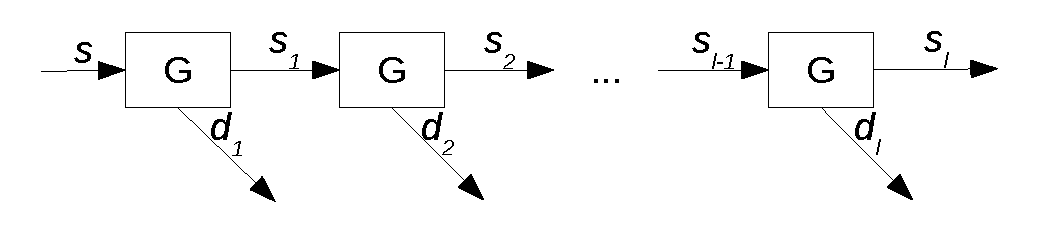
\includegraphics[width=0.8\linewidth]{drawings/prg-any-stretch.eps}
		\caption{Extending a \acs{PRG} with 1 bit stretch to a \acs{PRG} with $l$ bit stretch.}
		\label{fig:prg-any-stretch}
	\end{figure}

	First, let's look at the construction (\cref{fig:prg-any-stretch}).
	We replicate our \ac{PRG} $\G$ with 1 bit stretch $l$ times.
	The \ac{PRG} $\G^{l}$ that we define takes in input $s \in \{0,1\}^{\lambda}$, computes $(s_1, b_1) = \G(s)$, where $s_1 \in \{0,1\}^{l}$ and $b_1 \in \{0,1\}$, outputs $b_1$ and feeds $s_1$ to the second copy of \ac{PRG} $\G$, and so on until the $l$-th \ac{PRG}.

	To show that our construction is a \ac{PRG}, we define $l$ hybrids, with $\H_0^{\lambda} \equiv \G^{l}(\U_{\lambda})$, where $\G^{l} : \{0,1\}^{\lambda} \to \{0,1\}^{\lambda + l}$ is our proposed construction, and $\H_i^{\lambda}$ takes $b_1, \dots, b_i \rand{\{0,1\}}$, $s_i \rand{\{0,1\}^{\lambda}}$, and outputs $(b_1, \dots, b_i, s_l)$, where $s_l \in \{0,1\}^{\lambda + l - i}$ is $s_l = \G^{l-i}(s_i)$, \ie the output of our construction restricted to $l-i$ units.

	$\H_l^{\lambda}$ takes $b_1, \dots, b_l \rand{\{0,1\}}$ and $s_l \rand{\{0,1\}^{l}}$ and outputs $(b_1, \dots, b_l, s_l)$ directly.

	We need to show that $\H_i^{\lambda} \CompInd \H_{i+1}^{\lambda}$.
	To do so, fix some $i$.
	The only difference between the two hybrids is that $s_{i+1}, b_{i+1}$ are pseudo random in $\H_{i}^{\lambda}$, and are truly random in $\H_{i+1}^{\lambda}$.
	All bits before them are truly random, all bits after are pseudo random.

	Assume these two hybrids are distinguishable, then we can break the \ac{PRG}.
	Consider the \ac{PPT} function $f_i$ defined by $f(s_{i+1},b_{i+1}) = (b_1, \dots, b_l, s_l)$ such that $b_1, \dots b_i \rand{\{0,1\}}$ and, for all $j \in [i+1, l]$ $(b_j, s_j) = \G(s_{j-1})$.

	By the security of \acp{PRG} we have that $\G(\U_{\lambda}) \CompInd \U_{\lambda+1}$.
	By reduction, we also have that $f(\G(\U_{\lambda})) \CompInd f(\U_{\lambda+1})$.
	Thus, $\H_{i}^{\lambda} \CompInd \H_{i+1}^{\lambda}$.
\end{proof}

\subsection{\aclp{HCP}}

\begin{definition}[\acl{HCP} - I] \label{def:hcp-i}
	A polynomial time function $h : \{0,1\}^{n} \to \{0,1\}$ is \emph{hard core} for $f : \{0,1\}^{n} \to \{0,1\}^{n}$ if for all \ac{PPT} adversaries $\Adv$
	\begin{equation*}
		\Pr{\Adv(f(x)) = h(x) : x \rand{\{0,1\}^{n}}} \le \frac{1}{2} + \epsilon(\lambda).
	\end{equation*}
\end{definition}
The $\frac{1}{2}$ in the upper bound tells us that the adversary can't to better than guessing.

\begin{definition}[\acl{HCP} - II] \label{def:hcp-ii}
	A polynomial time function $h : \{0,1\}^{n} \to \{0,1\}$ is \emph{hard core} for $f : \{0,1\}^{n} \to \{0,1\}^{n}$ if for all \ac{PPT} adversaries $\Adv$
	\begin{equation*}
		\abs{
			\Pr{
			\begin{array}{c}
				\Adv(f(x), h(x)) = 1 : \\
				x \rand{\{0,1\}^{n}}
			\end{array}
			}
			-
			\Pr{
			\begin{array}{c}
				\Adv(f(x), b) = 1 : \\
				x \rand{\{0,1\}^{n}}; \\
				b \rand{\{0,1\}}
			\end{array}
			}
		}
		\le
		\epsilon(\lambda).
	\end{equation*}
\end{definition}

\begin{theorem}
	\Cref{def:hcp-i} and \cref{def:hcp-ii} are equivalent.
\end{theorem}
Proof of this theorem is left as exercise.

Luckily for us, every \ac{OWF} has a \ac{HCP}.
There isn't a single \ac{HCP} $h$ for all \acp{OWF} $f$.
Suppose $\exists$ such $h$, then take $f$ and let $f'(x) = h(x) || f(x)$.
Then, if $f'(x) = y || b$ for some $x$, it will always be that $h(x) = b$.

But, given a \ac{OWF}, we can create a new \ac{OWF} for which $h$ is hard core.

\begin{theorem}[\ac{GL}, 1983] \label{thm:gl}
	Let $f : \{0,1\}^n \to \{0,1\}^{n}$ be a \ac{OWF}, and define $g(x,r) = f(x) || r$ for $r \rand{\{0,1\}^{n}}$.
	Then $g$ is a \ac{OWF}, and 
	\begin{equation*}
		h(x,r) = \DotProduct{x}{r} = \sum_{i=1}^{n} x_i \cdot r_i \mod 2
	\end{equation*}
	is hardcore for $g$. 
\end{theorem}

\begin{definition}[\acl{OWP}]
	We say that $f : \{0,1\}^n \to \{0,1\}^{n}$ is a \ac{OWP} if $f$ is a \ac{OWF}, $\forall x . \abs{x} = \abs{f(x)}$, and for all distinct $x, x' . f(x) \neq f(x')$.
\end{definition}

\begin{corollary} \label{cor:owp-hcp-prg}
	Let $f$ be a \ac{OWP}, and consider $g : \{0,1\}^n \to \{0,1\}^{n}$ from the \ac{GL} theorem.
	Then $\G(s) = (g(s), h(s))$ is a \ac{PRG} with stretch 1.
\end{corollary}

\begin{proof}[Proof of \cref{cor:owp-hcp-prg}]
	\begin{align*}
		\G(\U_{2n})
		& =
		(g(x,r), h(x,r)) \\
		& =
		(f(x) || r, \DotProduct{x}{r}) \\
		& \CompInd 
		(f(x) || r, b) \tag{\ac{GL}}
		\\
		& \CompInd
		\U_{2n+1}.
	\end{align*}
\end{proof}

% this part is not clear

{\bfseries UNCLEAR}

Assume instead $f$ is a \ac{OWF}, and that is 1-to-1 (injective).
Consider $\X = g^m(\vec{x}) = (g(x_1), h(x_1), \dots, g(x_m), h(x_m))$, where $x_1, \dots, x_m \in \{0,1\}^{n}$ (\ie, $\vec{x} \in \{0,1\}^{nm}$).
You can construct a \ac{PRG} from a \ac{OWF} as shown by H.I.L.L.

\begin{fact}
$\X$ is indistinguishable from $\X'$ such that $\H_{\infty}(\X') \ge k = n \cdot m + m$, since $f$ is injective.
\end{fact}

Now $\G(s, \vec{x}) = (s, \Ext(s, g^{m}(\vec{x})))$ where $\Ext : \{0,1\}^{d} \times \{0,1\}^{nm} \to \{0,1\}^{l}$, and $l = nm + 1$.
This works for $m = \omega(\log(n))$.
You get extraction error $\epsilon \approx 2^{-m}$.

